\documentclass[stu, 12pt, letterpaper, donotrepeattitle, floatsintext, natbib]{apa7}
\usepackage[utf8]{inputenc}
%\usepackage{fontspec} %paquete para usar la fuente Arial 12
\usepackage{comment}
\usepackage{marvosym}
\usepackage{graphicx}
\usepackage{float}
\usepackage[normalem]{ulem}
\usepackage[spanish]{babel} 
\usepackage{lastpage} %para le formato que quiere la profe QUITAR SI QUIERES OG APA7
\usepackage{ragged2e} %para le formato que quiere la profe QUITAR SI QUIERES OG APA7
\usepackage{indentfirst} %para le formato que quiere la profe QUITAR SI QUIERES OG APA7

\setcounter{secnumdepth}{0} %permite enumerar las secciones QUITAR SI QUIERES OG APA7

%comando para ajustar la fuente Arial en todo el documento
%\setmainfont{Arial} %COMPILAR DOC CON XeLateX DOS VECES

\DeclareCaptionLabelSeparator*{spaced}{\\[2ex]}
\captionsetup[table]{textfont=it,format=plain,justification=justified,
  singlelinecheck=false,labelsep=spaced,skip=1pt}

\selectlanguage{spanish}

\useunder{\uline}{\ul}{}
\newcommand{\myparagraph}[1]{\paragraph{#1}\mbox{}\\}

%\rfoot{Página \thepage \hspace{1pt} de \pageref{LastPage}}%QUITAR SI QUIERES OG APA7 
\rhead{} %QUITAR SI QUIERES OG APA7
\setcounter{secnumdepth}{3} %permite enumerar las secciones QUITAR SI QUIERES OG APA7
\setlength{\parindent}{1.27cm} %sangria forzada QUITAR SI QUIERES OG APA7

\renewcommand\labelitemi{$\bullet$}

\newcommand*\chem[1]{\ensuremath{\mathrm{#1}}}

\begin{document}
    %PORTADA
    \begin{titlepage}
        \begin{figure}[ht]
            \centering
            
\includegraphics[width=15cm]{logosITT.png}
        \end{figure}
        \centering
        {\Large Tecnológico Nacional de México\\Instituto Tecnológico de Tijuana\par}
        \vspace{1cm}
        {\Large SCD-1011SC6C Ingeniería de Software\par}
        \vspace{1cm}
        {\Large Unidad 1\par}
        \vspace{2cm}
        {\Large\bfseries Caso práctico 1\par}
        \vspace{2cm}
        {\large Dra. Martha Elena Pulido\par}
        \vfill
            {\large Abraham Jhared Flores Azcona, 19211640\par}
        \vfill
        {\large 25 de febrero de 2021}
    \end{titlepage}

% Índices
\pagenumbering{arabic}
    % Contenido
\renewcommand\contentsname{Contenido}
\tableofcontents

% Cuerpo 
    %NOTA: PARA CITAR ESTILO "Merts (2003)" usar \cite{<nombre_cita_bib>}
    %                        "(Metz, 1978)" usar \citep{<nombre_cita_bib>}
\newpage
\section{Análisis de la situación de la empresa}
Basado \begin{justifying}
    en las circunstancias:
    \begin{itemize}
        \item Existe tráfico de influencias por la facilidad de manipulación del dueño respecto a su parcialidad con sus trabajadores/familia.
        \item Los trabajadores no consideraban un término a largo plazo. Se terminaron aprovechando de la capacitación gratuíta que los proveedores les brindaban.
        \item Mala paga.
        \item No tienen afiliación oficial ante los servicios de salúd.
        \item Su rendimiento como empresa es del 40\%.
        \item No han variado sus productos en tres años.
        \item Falta de consenso al respecto del manejo del capital (sacrifican salarios sobre activos).
        \item Cajas puede entremañar los flujos de efectivo al no tener delegada la responsabilidad.
        \item No hay metas fijas debido a la falta de consenso sobre las metas de producción diarias.
        \item Se pueden hacer alianzas estratégicas debido a la alta alfluencia de hobres de negocios a dicha panadería.
    \end{itemize}\par
\end{justifying}
\vspace{\baselineskip}
\section{Determinación los requisitos que se necesitarían, y determinar el diagrama UML de los documentos actuales}
\begin{justifying}
   \begin{itemize}
    \item Explicar los puntos previamente detectados.
    \item Establecer firmemente los objetivos tanto para los dueños como para los empleados.
    \item Establecer el plan de acción sobre manejo de recursos y formalización de prestaciones para cumplir con la ley.
   \end{itemize}
\end{justifying}
El diagrama UML de los procesos actuales es el siguiente:
\begin{figure}[H]
    \caption{\emph{Diagrama UML del escrito adjunto\\}}
    \centering
    \smallskip
    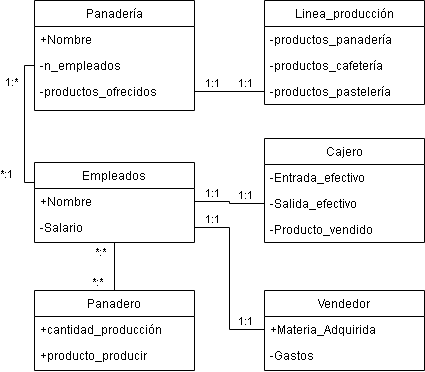
\includegraphics[width=14cm, height=10cm]{Untitled Diagram.drawio.png}
    \bigskip
    {\justifying\small\textit{\\Nota:} Autoría Propia (2022).}%citar al de medium del waterfall
\end{figure}
\vspace{\baselineskip}
\section{Conclusiones}
En \begin{justifying}
    este caso, dicho neocio debe de empezar a solidificar su estancia respecto a los objetivos que desean alcanzar y que tan factible deben de ser 
dichos objetivos para que todas las partes involucradas puedan seguir sosteniendo el empleo que ejercen. 
\end{justifying}
\end{document}